% Gemini theme
% See: https://rev.cs.uchicago.edu/k4rtik/gemini-uccs
% A fork of https://github.com/anishathalye/gemini

\documentclass[final]{beamer}

% ====================
% Packages
% ====================

\usepackage[size=custom,width=45,height=36,scale=0.5]{beamerposter}
\usetheme{gemini}
\usecolortheme{stanford}
\usepackage{graphicx}
\usepackage{booktabs}
\usepackage{tikz}
\usetikzlibrary{shapes, arrows, positioning, decorations.pathreplacing}
\usepackage{pgfplots}
\pgfplotsset{compat=1.17}
\usepackage{fontspec}
\usepackage{exscale}
\usepackage{tabularx}
\usepackage{colortbl} % For \rowcolor
\usepackage{xcolor}   % For color definitions
\usepackage{tcolorbox}
\usepackage[backend=biber, style=numeric-comp, maxnames=3, minnames=1, giveninits=true, uniquename=init]{biblatex}
\addbibresource{poster.bib} % Adjust the filename as needed
\usepackage{amssymb}

% Factor colors -- same hex values (and same 35%-tint-over-white rule, via
% xcolor's !35!white mixing) as diag_h2h3_forest.R's FACTOR_COLORS, so a
% factor reads as the same color here as in the H2/H3 forest plot.
\definecolor{factorCaregiverStress}{HTML}{7570B3}
\definecolor{factorEarlyResources}{HTML}{E6AB02}
\definecolor{factorNbhdSafety}{HTML}{D95F02}
\definecolor{factorEconHardship}{HTML}{E7298A}
\definecolor{factorHomeEnv}{HTML}{66A61E}
\definecolor{factorTrauma}{HTML}{A6761D}

% One factor's colored box: name in a fixed-width left column, its item
% list in the remaining width, both left-aligned -- an "invisible seam"
% since both columns share the box's own colback, no rule between them.
\newcommand{\factorbox}[3]{%
  \begin{tcolorbox}[colback=#1!35!white, colframe=#1!35!white,
    boxsep=1pt, top=2pt, bottom=2pt, left=4pt, right=4pt]
    \begin{minipage}[t]{0.32\linewidth}\textit{#2}\end{minipage}%
    \begin{minipage}[t]{0.66\linewidth}#3\end{minipage}
  \end{tcolorbox}}

% Banner colour options (from the upstream template README):
%   \setbeamercolor{headline}{bg=paloaltogreen,fg=white}  % white text, Palo Alto green banner
%   \setbeamercolor{headline}{bg=white,fg=cardinalred}    % cardinal red text, white banner
%   \setbeamercolor{headline}{bg=cardinalred,fg=white}    % white text, cardinal red banner
%   \setbeamercolor{headline}{bg=coolgray,fg=white}       % white text, cool grey banner
\setbeamercolor{headline}{bg=cardinalred,fg=white}
\setbeamercolor{footline}{bg=footergray,fg=darkcardinal}

% ====================
% More biblatex kwargs
% ====================

% Remove unnecessary fields
\AtEveryBibitem{
  \clearfield{issn}
  \clearfield{url}
  \clearfield{doi}
  \clearfield{eprint}
  \clearfield{urldate}
}

\AtEveryCitekey{\clearfield{urldate}}

\DeclareFieldFormat{urldate}{}

% Remove "visited on" date
\DefineBibliographyStrings{english}{
  urlseen = {}
}

% Reduce spacing between entries
\setlength{\bibitemsep}{0pt}

% Customize the way certain fields are printed
\DeclareFieldFormat[article]{title}{#1}
\DeclareFieldFormat[article]{volume}{\textbf{#1}}
\DeclareFieldFormat[article]{number}{(#1)}
\DeclareFieldFormat{pages}{#1}

% Customize the order and punctuation of fields
\renewbibmacro*{journal+issuetitle}{%
  \usebibmacro{journal}%
  \setunit*{\addspace}%
  \iffieldundef{series}
    {}
    {\newunit
     \printfield{series}%
     \setunit{\addspace}}%
  \usebibmacro{volume+number+eid}%
  \setunit{\addcolon\space}%
  \usebibmacro{issue+date}%
  \setunit{\addcomma\space}%
  \usebibmacro{issue}%
  \newunit}

\renewbibmacro*{volume+number+eid}{%
  \printfield{volume}%
  \printfield{number}%
  \setunit{\addcomma\space}%
  \printfield{eid}}

% ====================
% Lengths
% ====================

% If you have N columns, choose \sepwidth and \colwidth such that
% (N+1)*\sepwidth + N*\colwidth = \paperwidth
\newlength{\sepwidth}
\newlength{\colwidth}
\setlength{\sepwidth}{0.025\paperwidth}
\setlength{\colwidth}{0.3\paperwidth} % single continuous 3-column body, no row break

\newcommand{\separatorcolumn}{\begin{column}{\sepwidth}\end{column}}


\title{Does a Reproducible Promotive/Adversity Structure Exist in HBCD Infancy Data?}


\author{\fontsize{16}{18}\selectfont Howard Chiu \inst{1} \and Monica Ellwood-Lowe \inst{1} \and Philip Fisher \inst{1,2}}

\institute[shortinst]{%
  \inst{1} Graduate School of Education, Stanford University, Stanford, CA, USA \\
  \inst{2} Stanford Center on Early Childhood, Stanford University, Stanford, CA, USA
}

% ====================
% Footer (optional)
% ====================

\footercontent{
  \href{https://osf.io/9c4kt/overview}{OSF Preregistration: osf.io/9c4kt} \hfill
  Data provided by the HBCD Study, a consortium supported by NIH \hfill
  \href{mailto:howardchiu@stanford.edu}{howardchiu@stanford.edu}}


% ====================
% Body
% ====================

\begin{document}

% This adds the Logos on the top left and top right.
% Both nodes anchor to the same page corner type (north-*, which is the same
% y-coordinate on the page for west and east) with inner sep=3cm.

\addtobeamertemplate{headline}{}
{
  \begin{tikzpicture}[remember picture,overlay]
    \node [anchor=north west, inner sep=3cm] at ([xshift=-2.25cm,yshift=0.25cm]current page.north west)
    {
\includegraphics[width=6.25cm]{stanford_logos/GSE-hor-logo-white.png}};
  \end{tikzpicture}

  \begin{tikzpicture}[remember picture,overlay]
    \node [anchor=north east, inner sep=3cm] at ([xshift=18.70cm,yshift=2.25cm]current page.north east)
    {
\includegraphics[width=36.9cm]{stanford_logos/stanford-line2-10-white.png}};
  \end{tikzpicture}
}

\begin{frame}[t]
\vspace{-0.5cm}
\begin{columns}[t]
\separatorcolumn

\begin{column}{\colwidth}
  \begin{block}{HBCD's dense, longitudinal sampling lets us test reproducibility of factor structure across time}
    \vspace{-0.3cm}
    \begin{itemize}
      \setlength\itemsep{0.15em}
      \item Conceptual grounding: DMAP (dimensional model of
        adversity and psychopathology; threat vs.\ deprivation), unpredictability, 
        ecological systems theory (Bronfenbrenner), promotive vs.\
        protective factors.
      \item \textbf{Preregistered battery returned mostly null
        results.} Extended post-hoc with additional HBCD-collected
        measures (see Measures table) -- disclosed as a deviation.
    \end{itemize}

    \vspace{-0.4cm}
    \begin{tcolorbox}[colback=coolgray, colframe=coolgray, width=\linewidth]
      \color{white}
      \textbf{Q1 (H1)}: does a low-dimensional promotive/adversity
      structure exist in HBCD's item battery, and does it reproduce
      across independent subsets of the same cohort?

      \vspace{0.1cm}
      \textbf{Q2 (H2/H3)}: if so, do promotive-dominant dimensions
      predict more favorable outcomes, and do adversity-dominant
      dimensions protectively moderate that association?
    \end{tcolorbox}
  \end{block}

  \vspace{-0.5cm}
  \begin{block}{Two-stage design: discover, then confirm}
    \vspace{-0.2cm}
    \begin{itemize}
      \setlength\itemsep{0.15em}
      \item TP1 (prenatal-9mo) and TP2 (9-17mo) modeled independently
        via Bayesian EFA (BEFA). Rolling enrollment: TP2 N far smaller.
    \end{itemize}

    \vspace{-1.0cm}
    \begin{center}
    \resizebox{\linewidth}{!}{%
    \begin{tikzpicture}[node distance=2cm, auto]
      \tikzstyle{tp1block} = [rectangle, draw, fill=cardinalred,
        text width=4.4em, text centered, rounded corners,
        minimum height=3.4em, font=\small, text=white]
      \tikzstyle{tp2block} = [rectangle, draw, fill=paloaltogreen,
        text width=4.4em, text centered, rounded corners,
        minimum height=3.4em, font=\small, text=white]
      \tikzstyle{arrow} = [draw, thick, -latex']
      \tikzstyle{lbl} = [font=\normalsize, text centered]

      \node [tp1block] (tp1_n) {\textbf{\normalsize N=3{,}599}};
      \node [tp1block, right of=tp1_n, xshift=2.9cm] (tp1_disc) {\textbf{\normalsize Discovery\\ n=2{,}884}};
      \node [tp1block, right of=tp1_disc, xshift=3.1cm] (tp1_hold) {\textbf{\normalsize Holdout\\ n=715}};

      \node [tp2block, below of=tp1_n, yshift=0.4cm] (tp2_n) {\textbf{\normalsize N=682}};
      \node [tp2block, right of=tp2_n, xshift=2.9cm] (tp2_disc) {\textbf{\normalsize Discovery\\ n=558}};
      \node [tp2block, right of=tp2_disc, xshift=3.1cm] (tp2_hold) {\textbf{\normalsize Holdout\\ n=124}};

      \draw [arrow] (tp1_n) -- (tp1_disc) node [midway, above, lbl] {80\%};
      \draw [arrow] (tp1_disc) -- (tp1_hold) node [midway, above, lbl] {\shortstack{5-fold $\times$\\4-chain BEFA}};
      \draw [arrow] (tp2_n) -- (tp2_disc) node [midway, above, lbl] {80\%};
      \draw [arrow] (tp2_disc) -- (tp2_hold) node [midway, above, lbl] {\shortstack{5-fold $\times$\\4-chain BEFA}};

      \node [font=\bfseries, left of=tp1_n, xshift=-1.4cm] {TP1};
      \node [font=\bfseries, left of=tp2_n, xshift=-1.4cm] {TP2};
    \end{tikzpicture}%
    }
    \end{center}
    \vspace{-0.7cm}
    \begin{itemize}
      \setlength\itemsep{0.15em}
      \item 18 candidate items at TP1, 24 at TP2 (23 active --
        full list below).
    \end{itemize}
  \end{block}

  \vspace{-0.6cm}
  \begin{block}{Measures, visits, and timepoint assembly}
    \vspace{-0.1cm}
    \fontsize{9.5}{9.5}\selectfont
    \begin{tabularx}{\linewidth}{X r r r r r}
            \toprule
            & \multicolumn{3}{c}{TP1} & \multicolumn{2}{c}{TP2} \\
            \cmidrule(lr){2-4}\cmidrule(lr){5-6}
            \textbf{Measure} & \textbf{V01} & \textbf{V02} & \textbf{V03} & \textbf{V04} & \textbf{V05} \\
            \midrule
            Breastfeeding Hist.$^{\dagger *}$ & -- & 2255 & 64 & 9 & -- \\
            Area Depriv.\ Index (ADI)$^\dagger$ & 2649 & -- & -- & -- & 577 \\
            Child Opp.\ Index 2.0 (COI)$^\dagger$ & 2665 & -- & -- & -- & 580 \\
            MLDS (lang.\ exposure)$^\dagger$ & -- & -- & 1284 & 636 & -- \\
            Walkability Index$^\dagger$ & 2193 & -- & -- & -- & 467 \\
            Tree canopy cover$^\dagger$ & 2665 & -- & -- & -- & 580 \\
            Neighborhood safety$^\dagger$ & 3500 & 12 & -- & -- & 378 \\
            Econ.\ hardship: eviction$^\dagger$ & 3502 & 14 & -- & -- & 382 \\
            Econ.\ hardship: general$^\dagger$ & 3051 & 12 & -- & -- & 343 \\
            Food insecurity$^\dagger$ & -- & 2219 & 1312 & 627 & -- \\
            Transitions-in-Care$^\dagger$ & -- & 1057 & 743 & 521 & 52 \\
            E-HITS & 3395 & 12 & -- & -- & -- \\
            PhenX Discrimination$^\dagger$ & 3378 & 11 & -- & -- & 371 \\
            ecPROMIS CG-Child Rel.$^\dagger$ & -- & -- & 1323 & -- & 28 \\
            PACEs (current) & 3473 & 10 & -- & -- & -- \\
            PROMIS ES4a$^\dagger$ & 3507 & 2202 & 1302 & 629 & -- \\
            PSS-4$^\dagger$ & 3499 & 2203 & 1303 & 630 & -- \\
            IBQ-R (child temperament)$^\dagger$ & -- & -- & 1308 & -- & 352 \\
            ScreenQ (screen time) & -- & -- & -- & 641 & -- \\
            HOME Inv.: Cog.\ Stimulation & -- & -- & -- & 615 & -- \\
            PACEs (retrospective) & -- & -- & -- & -- & 382 \\
            HOME Inv.: Emotional Support & -- & -- & -- & 615 & -- \\
            CASR-SF (partner abuse) & -- & -- & -- & 530 & -- \\
            PEARLS (pediatric ACEs) & -- & -- & -- & 601 & -- \\
            ACEs (adult) & -- & -- & -- & 588 & -- \\
            ecPROMIS CG-Child Rel.$^\dagger$ & -- & -- & -- & -- & 392 \\
            CHAOS (unreflected) & -- & -- & -- & 634 & -- \\
            ECBQ (child temperament) & -- & -- & -- & -- & 74 \\
            \bottomrule
          \end{tabularx}

          \vspace{0.05cm}
          {\fontsize{9}{9.5}\selectfont\setlength{\parskip}{0pt}
          $^\dagger$ shared across timepoints (same instrument or
          GLED/PROMIS parallel form). $^*$ excluded at TP2, too sparse
          ($<$10\% coverage). Outcomes: 3 Bayley (cognitive/motor/
          language) subscales, CDI-WG (vocabulary),
          Vineland-ABC (adaptive behavior), PROMIS-Peer (peer
          relations), SPM-2 (sensory processing), MAP-DB (disruptive
          behavior). Covariates: site, maternal education/income,
          age.\par}
        \end{block}
      \end{column}

\separatorcolumn

\begin{column}{\colwidth}
  \begin{block}{No consistent factor structure for environmental variables}

    \begin{table}[ht]
      \centering
      \fontsize{13}{13.5}\selectfont
      \begin{tabularx}{\textwidth}{l c c c c}
        \toprule
        \textbf{Timepoint} & \textbf{Factors (M)} & \textbf{Folds agreeing} & \textbf{CFI (holdout)} & \textbf{RMSEA} \\
        \midrule
        TP1 & 4 & 3/5 -- \textbf{FAIL} & 0.903 (scaled) & 0.048 \\
        TP2 & 4 & 1/5 -- \textbf{FAIL} & 0.798 & 0.107 \\
        \bottomrule
      \end{tabularx}
    \end{table}
    \vspace{-0.25cm}
    \begin{itemize}
      \setlength\itemsep{0.1em}
      \item Held-out fit: TP1 fails CFI (0.903 vs.\ conventional threshold of 0.95) but clears
        RMSEA (0.048 vs.\ conventional threshold of 0.06); TP2 fails both (0.798, 0.107).
      \item Adding IBQ-R, GLED-TP2, and CHAOS post-preregistration changes item grouping but not instability.
    \end{itemize}

    \vspace{-0.7cm}
    \begin{figure}[ht]
      \centering
      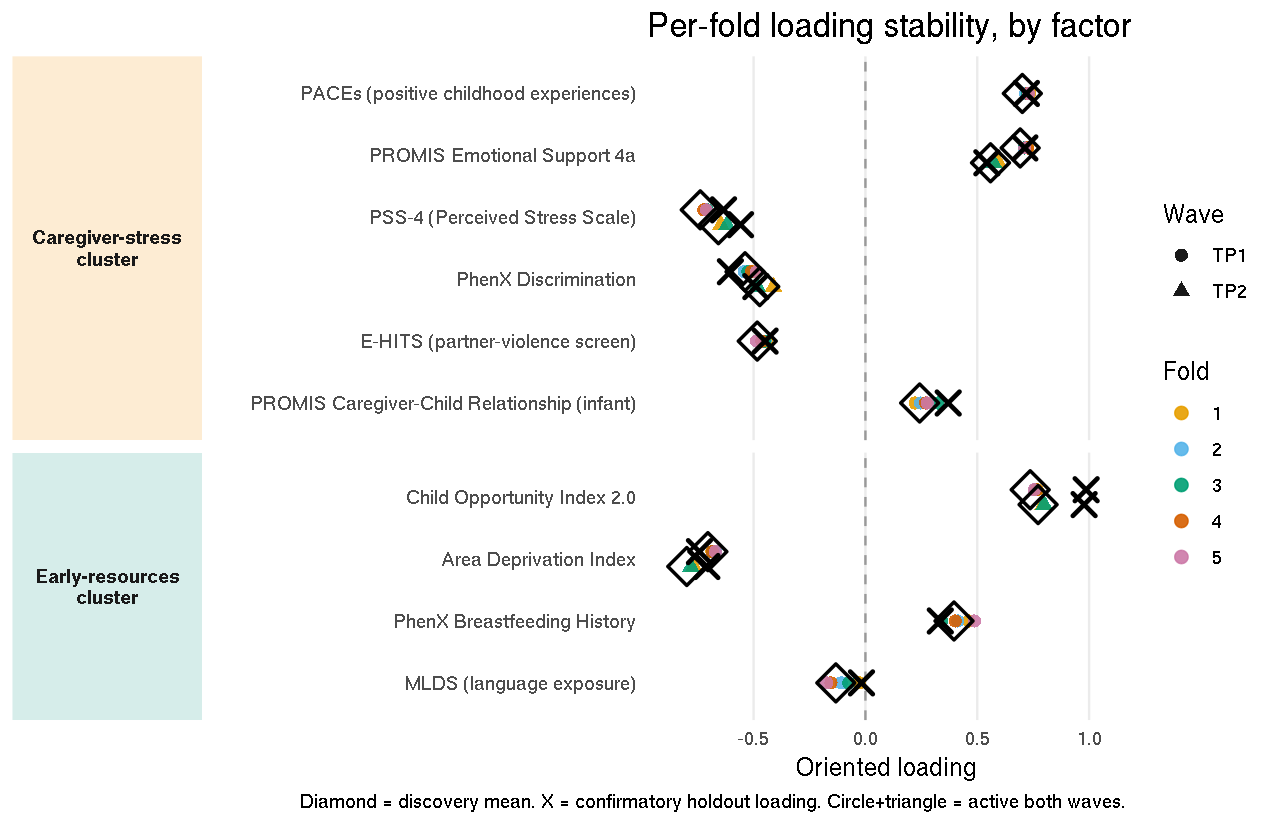
\includegraphics[width=0.85\textwidth]{figures/fold_loading_stability_adicoi_combined.png}
    \end{figure}
  \end{block}

  \vspace{-0.5cm}

  \begin{block}{Factor membership diverges between timepoints}
    \fontsize{12}{13.2}\selectfont
    % Each factor gets the same colored box (same hex, same 35% tint) as
    % its strip in the H2/H3 forest plot -- TP1 and TP2 are independent
    % stacks now (not a joined X X table row-for-row) since most factors
    % don't have a same-row counterpart in the other timepoint anyway.
    \begin{columns}[t]
      \begin{column}{0.49\linewidth}
        \centering\textbf{TP1}\\[3pt]
        \vspace{-0.3cm}
        \factorbox{factorEarlyResources}{Early-resources}{\mbox{COI+}, \mbox{ADI$-$}, \mbox{Breastfeeding+}, \mbox{MLDS$-$ (n.s.)}}
        \vspace{-0.5cm}
        \factorbox{factorCaregiverStress}{Caregiver-stress}{\mbox{PACEs+}, \mbox{ES4a+}, \mbox{PSS-4$-$}, \mbox{Discrimination$-$}, \mbox{E-HITS$-$}, \mbox{ecPROMIS+}, \mbox{IBQ-R$-$}}
        \vspace{-0.5cm}
        \factorbox{factorNbhdSafety}{Nbhd.-safety}{\mbox{Safety+}, \mbox{Eviction$-$}, \mbox{Tree canopy+}}
        \vspace{-0.5cm}
        \factorbox{factorEconHardship}{Econ.-hardship}{\mbox{Hardship+}, \mbox{Food insecurity+}}
      \end{column}
      \begin{column}{0.49\linewidth}
        \centering\textbf{TP2}\\[3pt]
        \vspace{-0.3cm}
        \factorbox{factorEarlyResources}{Early-resources}{\mbox{COI+}, \mbox{ADI$-$}}
        \vspace{-0.5cm}
        \factorbox{factorCaregiverStress}{Caregiver-stress}{\mbox{PSS-4$-$}, \mbox{Discrimination$-$}, \mbox{CHAOS$-$}, \mbox{ES4a+}}
        \vspace{-0.5cm}
        \factorbox{factorHomeEnv}{Home-env./ stimulation}{\mbox{HOME-ES+}, \mbox{HOME-CS+}, \mbox{PACEs(retro)+}, \mbox{Hardship$-$}, \mbox{ScreenQ$-$}, \mbox{Safety (n.s.)}}
        \vspace{-0.5cm}
        \factorbox{factorTrauma}{Trauma/ abuse-history}{\mbox{PEARLS+}, \mbox{CASR-SF+}, \mbox{ACEs(adult)+}}
      \end{column}
    \end{columns}

    \vspace{0.05cm}
    {\fontsize{11}{11.5}\selectfont\setlength{\parskip}{0pt}
    Signs = holdout loading direction (not magnitude); TP2 realigned to
    TP1's orientation where factors recur (ADI/COI,
    PSS-4/ES4a/Discrimination), since BEFA's sign is arbitrary per timepoint.
    n.s. = not significant.\par}
  \end{block}

  \vspace{-0.75cm}
  \begin{figure}[ht]
    \centering
    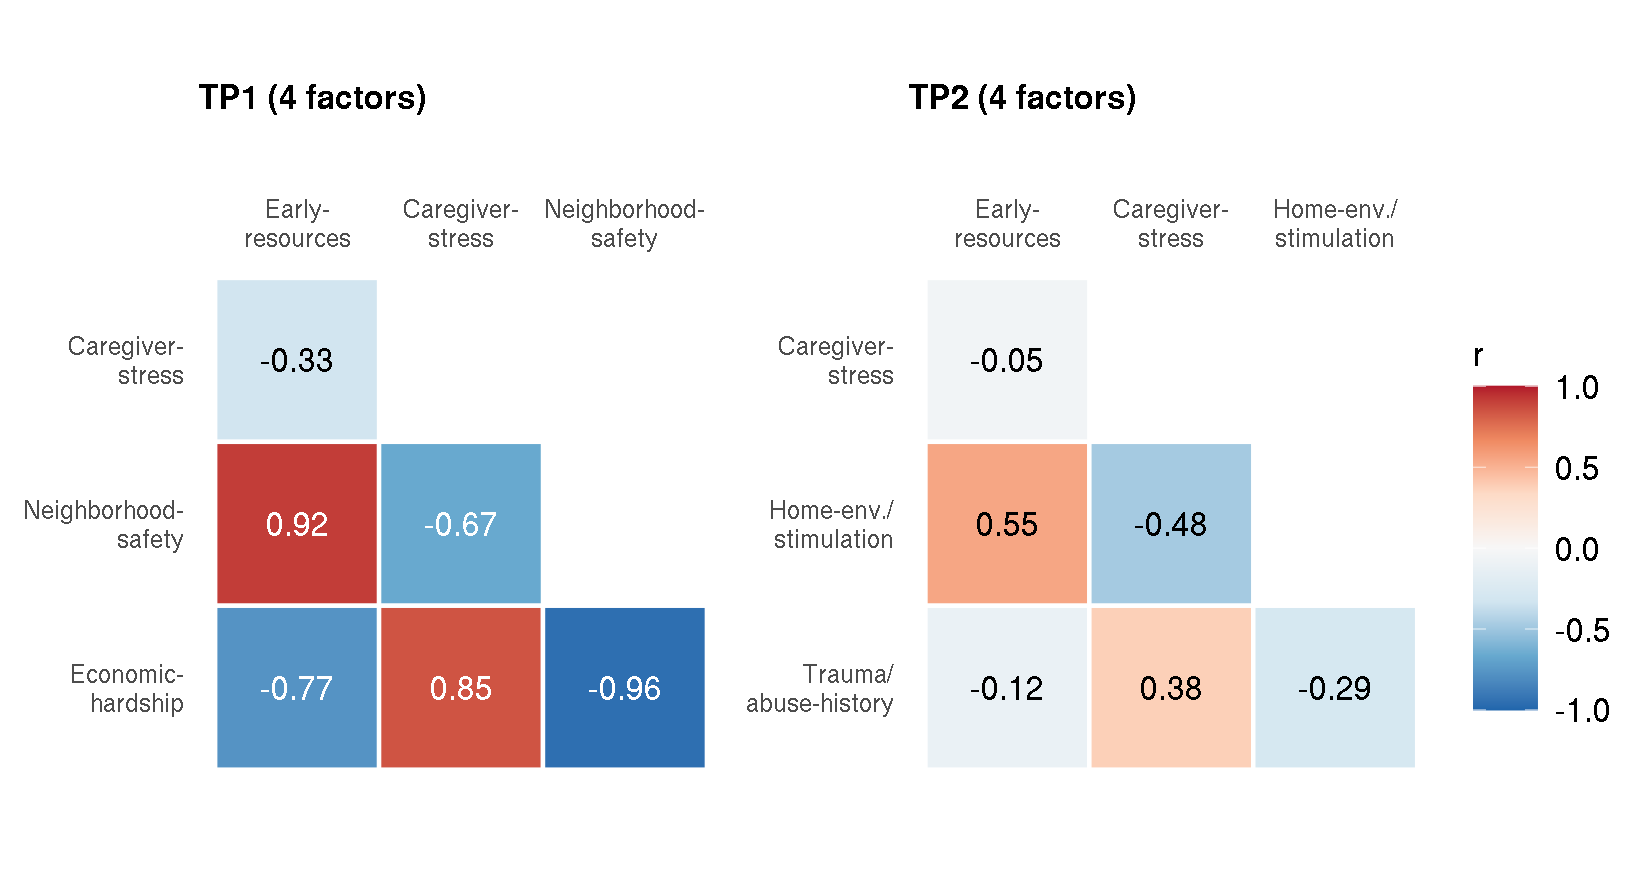
\includegraphics[width=0.85\textwidth]{figures/factor_correlation_heatmap.png}
  \end{figure}
\end{column}

\separatorcolumn

\begin{column}{\colwidth}
  \begin{block}{Absence of evidence for promotive/adversity--outcome effects}
    \vspace{-0.2cm}
    \textbf{H2}: outcome $\sim$ 4 factors + age + site, simultaneous.
    \\
    \textbf{H3}: H2 + each timepoint's clearest promotive $\times$ adversity
    interaction.

    \vspace{-0.35cm}
    \begin{figure}[ht]
      \centering
      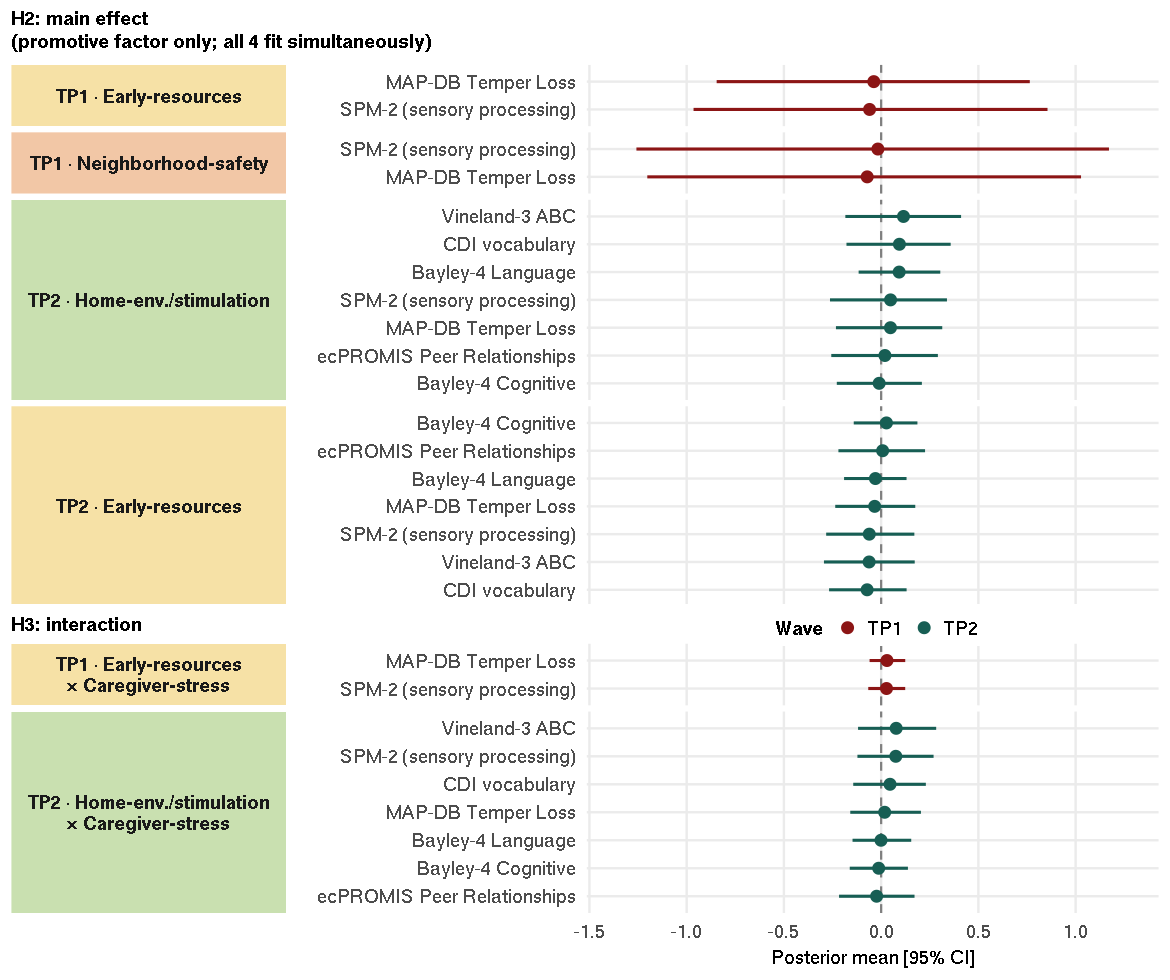
\includegraphics[width=0.7\textwidth]{figures/h2h3_forest_plot.png}
    \end{figure}
  \end{block}

  \vspace{-0.9cm}

  \begin{block}{TP1's Early-resources factor predicts fewer sensory/temper problems in marginal model}
    \vspace{-0.2cm}
    \textbf{Marginal (one-factor-at-a-time) models} -- drop every
    other factor covariate, keep age/site only:

    \vspace{-0.55cm}
    \begin{figure}[ht]
      \centering
      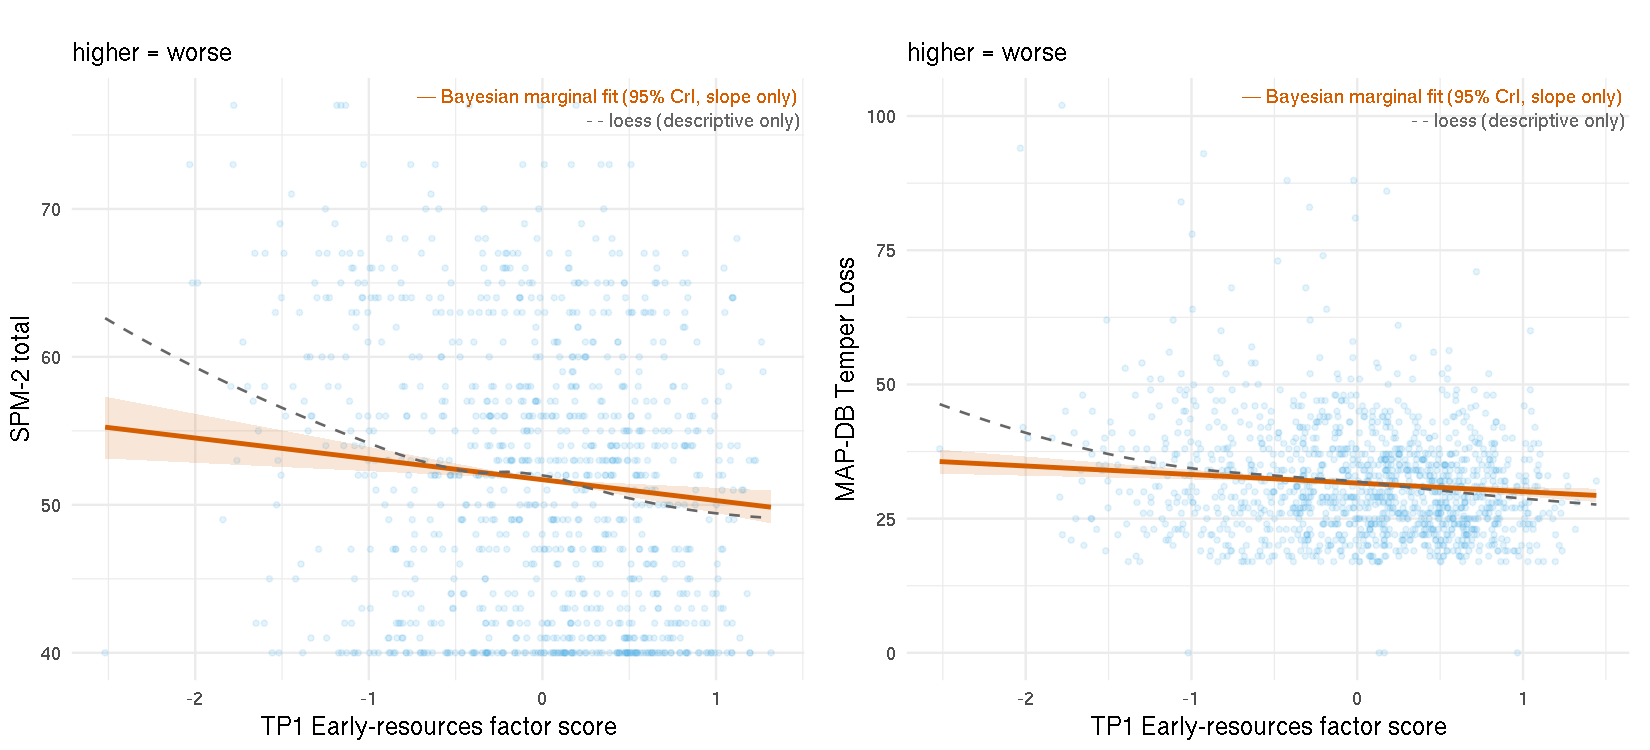
\includegraphics[width=0.75\textwidth]{figures/marginal_effect_scatter_tp1.png}
    \end{figure}
    \vspace{-0.5cm}
    \begin{itemize}
      \setlength\itemsep{0.1em}
      \item \textbf{The signal}: tested alone, this factor predicts
        fewer sensory-processing (SPM-2, $-0.155$) and temper-loss
        (MAP-DB, $-0.151$) problems.
      \item \textbf{Confounds explain only part of the signal}: TP1's
        only 2 outcomes are both caregiver-reported on nearly
        the same sample ($r=0.437$).
      \item \textbf{Cross-timepoint check}: shared items are
        adversity-heavy, model fit actually worse across chains and folds.
      \item \textbf{SES check}: partialling out maternal ed./income
        (+ site) doesn't shrink ADI/COI's correlation ($-0.69$ to
        $-0.73$) -- but shrinks breastfeeding/ language exposure's link
        to outcomes near zero.
    \end{itemize}
  \end{block}

  \vspace{-0.6cm}

  \begin{block}{Conclusions \& future directions}
    \vspace{-0.35cm}
      \begin{itemize}
        \setlength\itemsep{0.15em}
        \item Neither timepoint reproduced -- but ADI/COI's correlation
          stayed stable ($r=-0.69$ TP1, $-0.70$ TP2).
        \item Absence of evidence for H2/H3 association.
        \item TP1's factor collinearity limits independent signal from
          any one factor.
        \item \textbf{Food for thought}: neighborhood factors merge
          ($|r|$ up to 0.96), yet ADI/COI stay distinct from household
          items (SES check) -- nested (Bronfenbrenner) levels? Next:
          CFA, nested vs.\ single-factor, on holdout.
        \item \textbf{Next step}: as HBCD's rolling enrollment grows
          TP2's N, run a cross-timepoint measurement-invariance test on
          shared items to disambiguate developmental change vs.\ instrument-switching.
      \end{itemize}
  \end{block}

  \vspace{-0.3cm}

%  \begin{block}{References}
%    \renewcommand{\bibfont}{\fontsize{7}{9}\selectfont}
%    \printbibliography[heading=none]
%  \end{block}
\end{column}

\separatorcolumn
\end{columns}
\end{frame}
\end{document}